\subsection{Baglin, Collins, Gröbner, Grünhagel et al. 2001 (CERN)}
\label{sec:Baglin2}
Photon-induced scrubbing is quantified with the same measurement apparatus as presented in Sec.~\ref{sec:Baglin}~\cite{baglin2}.
Again, co-laminated copper with and without sawtooth was subject of these studies, however only the results for the material with included sawtooth are fully reported.

\subsubsection{Experiment setup}
Copper samples were irradiated with light from the Electron-Positron Accumulator (EPA, now dismantled) and their reflectivities and photoelectron yields were measured in the same way as in Sec.~\ref{sec:Baglin}.
The sample consisted of a Cu sawtooth structure.


\subsubsection{Results}

Figure~\ref{fig:baglin2_scrubbing} shows the results from the measurements of this paper.
There are clear differences in the reflectivity, which is much higher than in Fig.~\ref{fig:baglin_table}.
This implies that the yield is much smaller and the reflectivity much higher than before.
Furthermore they document the photon scrubbing after a dose of 1.5~$\cdot10^{22}$ photons, corresponding to about 600~h of LHC operations, as stated in the paper.
After this, the yield is about halved.
However the full results indicate that this process has not even saturated and could possibly be going even further, see Fig.~\ref{fig:baglin2_scrubbing}.
There seems to be no effect on the reflectivity.

\begin{figure}[tbh]
    \centering
    \begin{minipage}[c]{0.37\textwidth}
        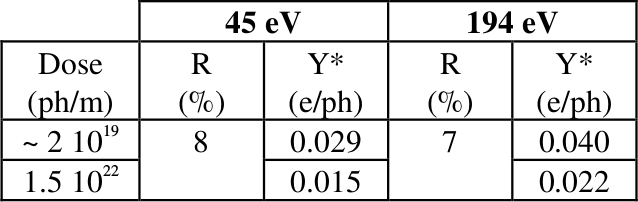
\includegraphics[width=\textwidth]{../ss/experiment_baglin2.png}
    \end{minipage}
    \hspace{0.5cm}
    \begin{minipage}[c]{0.57\textwidth}
        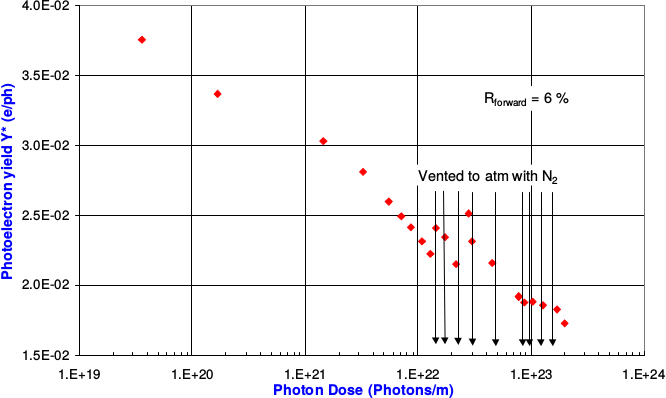
\includegraphics[width=1\textwidth]{../ss/photoelectron_scrubbing_baglin2.png}
    \end{minipage}
    \caption{
        Left: the reflectivities and photoelectron yields from the measurements of Copper samples with sawtooth presented in Sec.~\ref{sec:Baglin2}.
        \\
        Right: the impact of photon scrubbing on the photoelectron yield.
    }
    \label{fig:baglin2_scrubbing}
\end{figure}


The differences to the paper discussed in Sec.~\ref{sec:Baglin}, performed with the same experiment setup, is explained with the conditioning by reflected photons during the previous experiments.

\subsubsection{Open questions}

\begin{enumerate}
    \item It is stated that Cu co-lam. without sawtooth has been subject to this study as well, yet these results are not published.
\end{enumerate}

